\documentclass[12pt,fleqn]{article}\usepackage{../../common}
\begin{document}
Green'in Teorisi, Düzlem Kesişmeleri, Eğriler

Çizgi Düzlem Kesişmesini Vektörler ile Hesaplamak

Üstteki yöntem cebirsel manipülasyon gerektiriyor, fakat sayısal hesap için
sembolik cebir işlemlerine girmeden vektör matematiği ile direk bir sonuç
bulamaz mıyız? [3,4]'ü temel alalım: alttaki durumu düşünelim, 

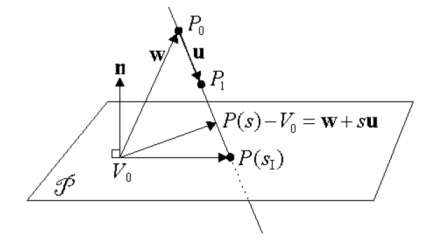
\includegraphics[width=20em]{calc_multi_75_app_06.jpg}

Grafiğe göre $P(s)$ $P_1$ ve $P_0$ arasındaki birim vektörün $s$ kadar
uzatılmış hali olsun, o aralığı $u$ kabul edersek $P(s)-V_0 = w + su$
olur. Düzlem ile kesişmenin olduğu noktayı $P(s_I)$ diye tanımlayalım,
aradığımız nokta burası. O noktada $n$ ile $P(s_I)$ dikgen olacaktır, yani
$P(s) - V_0 = w + su$ vektörü $n$'e dikgen olacaktır, ki $w=P_0-V_0$. Bu
durumda $n \cdot (w+su) = 0$ olur. Bunu kullanarak,

$$ s_I = \frac{-n \cdot w}{n \cdot u} = 
\frac{n \cdot (V_0 - P_0)}{n \cdot (P_1-P_0)} = 
\frac{-(ax_0 + by_0 + cz_0 + d)}{n \cdot u}
$$

\begin{minted}[fontsize=\footnotesize]{python}
n = np.array([1., 1., 1.])
V0 = np.array([1., 1., -5.])
P0 = np.array([-5., 1., -1.])
P1 = np.array([1., 2., 3.])

w = P0 - V0;
u = P1-P0;
N = -np.dot(n,w);
D = np.dot(n,u)
sI = N / D
I = P0+ sI*u
print I
\end{minted}

\begin{verbatim}
[-3.90909091  1.18181818 -0.27272727]
\end{verbatim}

Grafiklersek

\begin{minted}[fontsize=\footnotesize]{python}
import sys; sys.path.append('../../vision/vision_02')
import plot3d

f = plt.figure()
ax = f.gca(projection='3d')
w = 10
ax.set_xlim(-w,w);ax.set_ylim(-w,w);ax.set_zlim(-w,w)
ax.set_xlabel("X")
ax.set_ylabel("Y")
ax.set_zlabel("Z")
v = P1-P0
ax.quiver(P0[0], P0[1], P0[2], v[0], v[1], v[2], color='red')
ax.scatter(V0[0], V0[1], V0[2], color='black')
ax.scatter(V0[0]+n[0], V0[1]+n[1], V0[2]+n[2], color='black')
ax.scatter(I[0], I[1], I[2], color='black')
ax.quiver(V0[0], V0[1], V0[2], n[0], n[1], n[2], color='blue')
plot3d.plot_plane(ax, list(V0), list(n), color='y')
plt.savefig('calc_multi_75_app_07.jpg')
\end{minted}

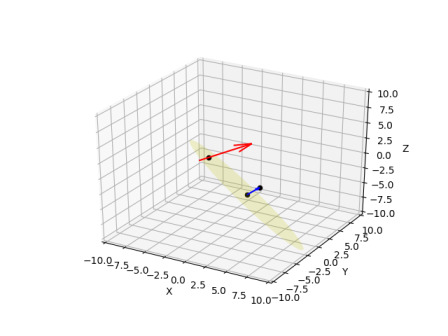
\includegraphics[width=20em]{calc_multi_75_app_07.jpg}

Green'in Teorisi, Uzaklaşım, Stokes, Yol ve Çizgi Entegralleri

Yüzeyler (Surfaces)

Üç boyut içindeki iki boyut yüzeyler parametrize edilerek gösterilir,
tek boyutlu eğri bir parametre $t$ ile parametrize ediliyordu, alan için
iki değişken $u,v$ gerekir. Notasyonel olarak $r$'nin taradığı bir yüzey

$$
r(u,v) = < x(u,v), y(u,v), z(u,v) >
$$

Mesela $r(u,v) = < u, u^2, v >$ bir yüzey olabilir.

Yüzey alan hesabı için tüm yüzeyi kenarları $\Delta u$, $\Delta v$ olan hücreler
yaratabiliriz. Her noktada iki tane teğet vektör bulunabilir, bunlar $t_u$ ve
$t_v$ olsun,

$$
t_u = < \frac{\partial x}{\partial u},
        \frac{\partial y}{\partial u},
        \frac{\partial z}{\partial u} >, \quad
t_v = < \frac{\partial x}{\partial v},
        \frac{\partial y}{\partial v},
        \frac{\partial z}{\partial v} >        
$$

Yaklaşık olarak her hücrenin alanı $\Delta S_{ij}$ her hücredeki $t_u$ ve $t_v$
(ya da yeni notasyonla onlara $t_u^{ij}$ ve $t_v^{ij}$ diyelim) yönündeki
$\Delta u$ ve $\Delta v$'nin oluşturduğu paralelogram alanıdır, bu paralelogram
bildiğimiz gibi iki vektörün çapraz çarpımından gelen üçüncü vektörün
büyüklüğüdür, o zaman 

$$
\Delta S_{ij} \approx || \Delta u t_u^{ij} \times \Delta v t_v^{ij} ||
$$

$$
= ||  t_u^{ij} \times t_v^{ij} || \Delta u \Delta v
$$
        
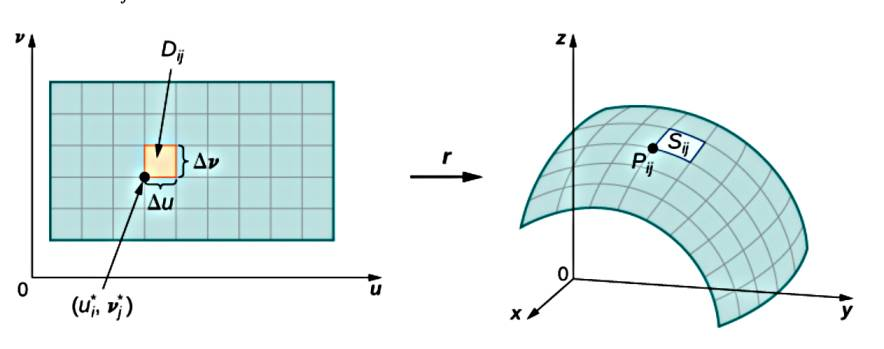
\includegraphics[width=20em]{calc_multi_75_app_01.jpg}

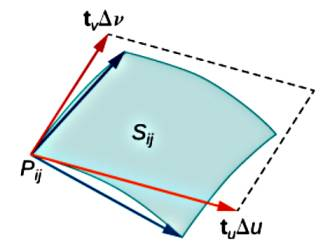
\includegraphics[width=10em]{calc_multi_75_app_02.jpg}

Tüm ufak hücre alanlarını toplarız, ve hücre sayısı sonsuza yaklaşırken toplam
alan limitine bakabiliriz,

$$
\lim_{m,n \to \infty} \sum_{i=1}^{m} \sum_{j=1}^{n} || t_u^{ij} \times t_v^{ij} || \Delta u \Delta v
$$

Bu limit yüzey alan çift entegral hesabına yaklaşır / onu tanımlar, [2, sf. 769],

$$
= \iint_D || t_u \times t_v || \ud u \ud v = \iint_D || t_u \times t_v || \ud A
$$

Yüzey Entegrali (Surface Integral)

Yukarıda gördüklerimiz parametrize edilmiş yüzeyin alanını hesaplamak içindir.
Yüzey entegrali bir yüzey {\em üzerinden} alınan entegrallere verilen isimdir,
mesela tek sayı / skalar değerli bir fonksiyon $f$'nin pürüzsüz bir yüzey $S$
üzerinden alınan yüzey entegrali, o fonksiyonun her noktadaki alan büyüklüğü ile
çarpılıp sonuçların toplanmasıdır, cebirsel olarak yine $t_u,t_v$ kavramlarını
kullanırsak,

$$
\iint_S f(x,y,z) \ud S 
= \lim_{m,n \to \infty} \sum_{i=1}^{m} \sum_{j=1}^{n} f(P_{ij}) || t_u^{ij} \times t_v^{ij} || \Delta u \Delta v
$$

$$
= \lim_{m,n \to \infty} \sum_{i=1}^{m} \sum_{j=1}^{n} f(P_{ij}) \Delta S_{ij} 
$$

O zaman yüzey entegralleri alttaki şekilde hesaplanabilir,

$$
\iint_S f(x,y,z) \ud S =
\iint_D f(r(u,v)) || t_u \times t_v || \ud A
$$

Çizgi entegrali (line integrals) daha düşük boyuttaki benzer bir kavram idi.

Vektör Alanları Üzerinden Yüzey Entegrali

Skalar fonksiyona benzer şekilde bir vektör alanı $F$ ve yüzey $S$ üzerinden de
entegral hesaplanabilir. Yine bir ufak çarpımlar toplamından bahsediyoruz, bu
tür bir hesap pek çok uygulama için faydalı olabilir. Mesela bir su akışı
içindeki geçirgen bir yüzeyi düşünürsek, kütle akışını (mass flux) nasıl
hesaplarız? 

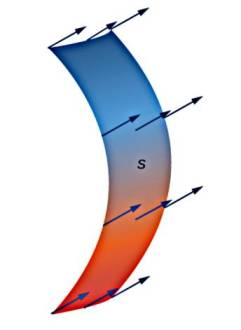
\includegraphics[width=10em]{calc_multi_75_app_04.jpg}

Her noktada yüzey $S$'ye dik olan alan $N$ olsun, her noktadaki akış hızı $v$
diyelim, o zaman bir noktadaki birim zaman ve birim alandaki kütle akışı $\rho v
\cdot N$. Ölçüm birimlerini kontrol edelim, hız $m/s$, yoğunluk $\rho$ 
$g/m^3$, çarparsak $g/s \cdot m^2$ elde ederiz, yani birim alan ve zamandaki
kütle akışı.

Şimdi $\rho v \cdot N$ değerini $\Delta S_{ij}$ ile çarparsak $S$ üzerindeki
hayali ufak hücreden birim zamanda akan kütleyi buluruz, tüm bu akışları
toplarız,

$$
\sum_{i=1}^{m} \sum_{j=1}^{n} (\rho v \cdot N) \Delta S_{ij}
$$

Tüm akışı elde etmiş oluruz. Izgara hücreleri $S_{ij}$ ufaldıkça üstteki toplam
gerçek kütle akışına yaklaşır, yani

$$
\iint_S \rho v \cdot N \ud S = \lim_{m,n \to \infty}
\sum_{i=1}^{m} \sum_{j=1}^{n} (\rho v \cdot N) \Delta S_{ij}
$$

Devam edelim $\rho v$ yerine herhangi bir vektör alanı $F$ kullanalım, o zaman
şu genel tanımı artık yapabiliriz, $F$'nin $S$ yüzeyi üzerinden entegrali

$$
\iint_S \vec{F} \cdot \ud \vec{S} = \iint_S \vec{F} \cdot \vec{N} \ud S
$$

olarak gösterilir.

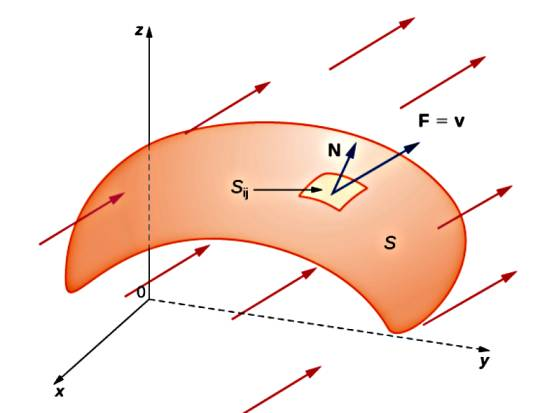
\includegraphics[width=15em]{calc_multi_75_app_05.jpg}

Dikkat her yerde vektör notasyonu kullanmıyoruz, olmadığı yerde formül
çerçevesine göre anlaşılabilir.

$N$ yüzey normalı, öne dik olan birim vektör, hesabı için önceden gördüğümüz
$t_u,t_v$ vektörlerini kullanabiliriz,

$$
N = \frac{t_u \times t_v}{ || t_u \times t_v || }
$$

Üstteki ifadeyi yüzey entegralinde kullanırsak [2, sf. 778],

$$
\iint_S \vec{F} \cdot \vec{N} \ud S =
\iint_S \vec{F} \cdot \frac{t_u \times t_v}{ || t_u \times t_v || } \ud S
$$

Daha önce gördük

$$
\ud S = || t_u \times t_v || \ud u \ud v = || t_u \times t_v || \ud A
$$

İki üste geçirince

$$
= \iint_D \vec{F}(r(u,v)) \cdot \frac{t_u \times t_v}{ || t_u \times t_v || }
|| t_u \times t_v || \ud A
$$

Basitleştirme sonrası,

$$
= \iint_D \vec{F}(r(u,v)) \cdot (t_u \times t_v) || t_u \times t_v || \ud A
$$

Soru

$F = < -y, x, 0 >$ olarak veriliyor, $S$ yüzeyi $r(u,v) = < u, v^2 - u, u+v >$.

$\iint_S F \cdot N \ud S$ yüzey entegralini hesaplayın.

Cevap

Teğet vektörler $t_u = < 1, -1, 1 >$, ve $t_v = < 0, 2v, 1 >$.

$t_u \times t_v$ çapraz çarpımı

\begin{minted}[fontsize=\footnotesize]{python}
import sympy

u,v = sympy.symbols('u v')
t_u = sympy.Matrix([[1,-1,1]])
t_v = sympy.Matrix([[0,2*v,1]])
print (t_u.cross(t_v))
\end{minted}

\begin{verbatim}
Matrix([[-2*v - 1, -1, 2*v]])
\end{verbatim}

Yüzey entegral hesabı şöyle hesaplanabilir,

$$
\int _{0}^{4} \int _{0}^{3} F(r(u,v)) \cdot (t_u \times t_v) \ud u \ud v
$$

Verili $F = < -y, x, 0 >$, ve yüzey $r(u,v) = < u, v^2 - u, u+v >$ demiştik,
o zaman 

$$
F(r(u,v)) = < u-v^2, u, 0 > 
$$

olur. Tüm entegral

$$
= \int _{0}^{4} \int _{0}^{3} < u-v^2, u, 0 >  \cdot < -1-2v, -1, 2v >
\ud u \ud v
$$

$$
= \int_{0}^{4} \int_{0}^{3} (2v^3 + v^2 -2uv -2u )
\ud u \ud v
$$

$$
= \int_{0}^{4} [ 2v^3u + v^2u - vu^2 - u^2 ]_{0}^{3} \ud v
$$

$$
= \int_{0}^{4} (6v^3 + 3v^2 - 9v -9 ) \ud v
$$

$$
= \left[ \frac{3v^4}{2} + v^3 - \frac{9v^2}{2} - 9v \right]_{0}^{4}
$$

$$
= 340
$$

\begin{minted}[fontsize=\footnotesize]{python}
from mpl_toolkits.mplot3d import Axes3D
from matplotlib import cm
import numpy as np
fig = plt.figure()
ax = fig.add_subplot(111, projection='3d')
u = np.linspace(0, 3, 100)
v = np.linspace(0, 4, 100)
u,v = np.meshgrid(u,v)

x = u; y = v**2 - u; z = u + v

ax.plot_surface(x, y, z, rstride=4, cstride=4, cmap = cm.copper)
x = np.linspace(0, 3, 5)
y = np.linspace(0, 10, 5)
z = np.linspace(0, 6, 5)

fu = -y; fv = x; fw = z*0

xx,yy,zz = np.meshgrid(x,y,z)
ax.quiver(xx, yy, zz, fu, fv, fw, length=0.2, color = 'red')
ax.view_init(elev=18, azim=-46)
plt.savefig('calc_multi_75_app_03.jpg',quality=30)
\end{minted}

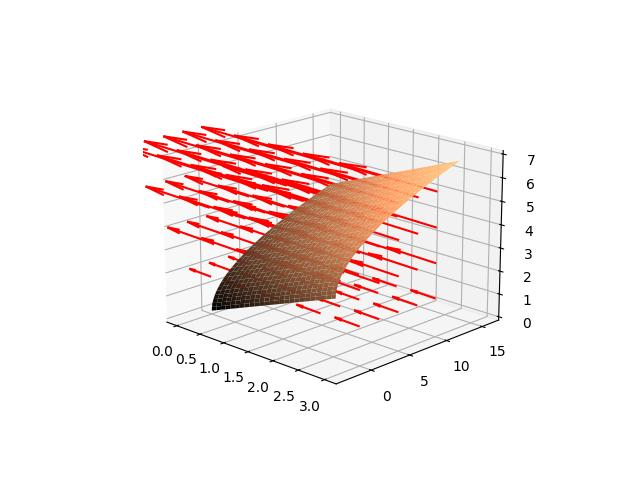
\includegraphics[width=15em]{calc_multi_75_app_03.jpg}

Çizgi Düzlem Kesişmesi

Elimizde $P = 2x + y - 4z = 4$ düzlemi var. Bu düzlemin 

$$ x = t \quad y = 2 + 3t \quad z = t$$

çizgisi ile kesiştiği yer neresidir? 

Cevap kolay; çizgi denkleminde $t$ bazlı tanımlı $x,y,z$ değerleri $P$'ye
sokarsak, tek bilinmeyeni $t$ olan bir denklem çıkar, 

$$ 2(t) + (2+3t)-4(t) = 4 \Rightarrow t = 2$$

İki Nokta Arasında Parametrize Edilmiş Eğri

Diyelim ki $(1,1)$ ve $(4,4)$ noktalarından geçen ve dışarıdan tanımlı
parametrelerle yeterince eğilip, bükülebilecek bir eğri tanımlamamız
lazım. Polinomlar üzerinden tanımlanan bir eğri ile bunu başarabiliriz, 

$$
x(t) = a_0 + a_1 t + a_2 t^2 + a_3 t^3
$$

$$
y(t) = b_0 + b_1 t + b_2 t^2 + b_3 t^3
$$

Bu şekilde bir eğri yeterince eğilip bükülebilir, ve istenen şekle
sokulabilir. Fakat baş ve sonun verili noktalardan geçmesini nasıl garanti
ederiz? Bunun için bu noktaları üstteki denkleme sokalim, ve $0 \le t \le
1$ olacak sekilde kısıtlama yapalim, $t=0$'da

$$
1 = a_0 + a_1 (0) + a_2 (0)^2 + a_3 (0)^3
$$

$$
1 = b_0 + b_1 (0) + b_2 (0)^2 + b_3 (0)^3
$$

Yani  $a_0=1$ ve $b_0=1$. Peki $t=1$ icin?

$$
4 = 1 + a_1 (1) + a_2 (1)^2 + a_3 (1)^3 
$$

$$
4 = 1 + b_1 (1) + b_2 (1)^2 + b_3 (1)^3 
$$

$$
3 = a_1 + a_2 + a_3, \quad 3 = b_1 + b_2 + b_3
$$

Demek ki üstteki iki formüle mutabık kaldığımız sürece
$a_1,a_2,a_3,b_1,b_2,b_3$ ie istediğimiz şekilde oynayarak istediğimiz
eğriyi ortaya çıkartabiliriz. 

\begin{minted}[fontsize=\footnotesize]{python}
t = np.linspace(0,1.0,100)

a1,a2 = -1.1, 1.9
b1,b2 = 1.1, 1.4

sx,sy=(1.0,1.0)
ex,ey=(4.0,4.0)

a3 = ex - sx - (a1+a2)
b3 = ey - sy - (b1+b2)

x = 1.0 + a1*t + a2*t**2 + a3*t**3
y = 1.0 + b1*t + b2*t**2 + b3*t**3

plt.xlim(0,5.0)
plt.ylim(0,5.0)
plt.plot(x,y)
plt.savefig('calc_multi_75_app_08.jpg')
\end{minted}

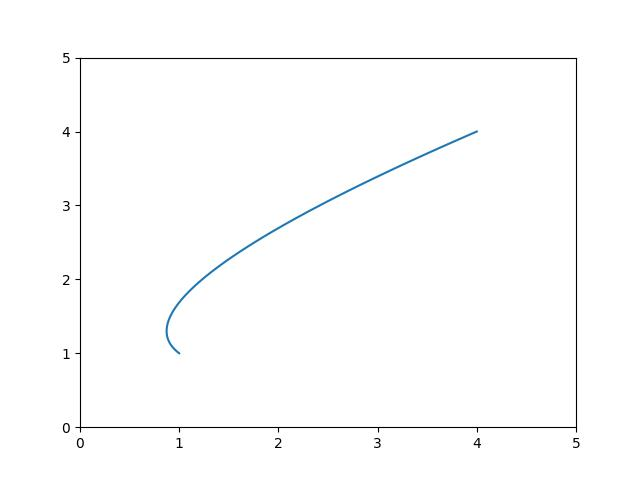
\includegraphics[width=20em]{calc_multi_75_app_08.jpg}

Max ve Sigmoid Bazlı Yaklaşım

Daha önce [6]'da görülen spline tekniğinin parametrik hali de
olabilir. Mesela 

\begin{minted}[fontsize=\footnotesize]{python}
a1,b1,c1,d1 = (1, -1.4, 2, 2.5)
a2,b2,c2,d2 = (1, 1.4, 1, 2.5)
def f(t):
    x = ax + \
        bx*np.max([0,t-2]) + \
        cx*np.max([0,t-3]) + \
        dx*np.max([0,t-4])
	   
    y = ay + \
        by*np.max([0,t-2]) + \
        cy*np.max([0,t-3]) + \
        dy*np.max([0,t-4])
    return x,y	   
    
tmp = np.linspace(0,5,100)
res = np.array([f(tt) for tt in tmp])
plt.plot(res[:,0],res[:,1])
plt.savefig('calc_multi_75_app_09.jpg')
\end{minted}

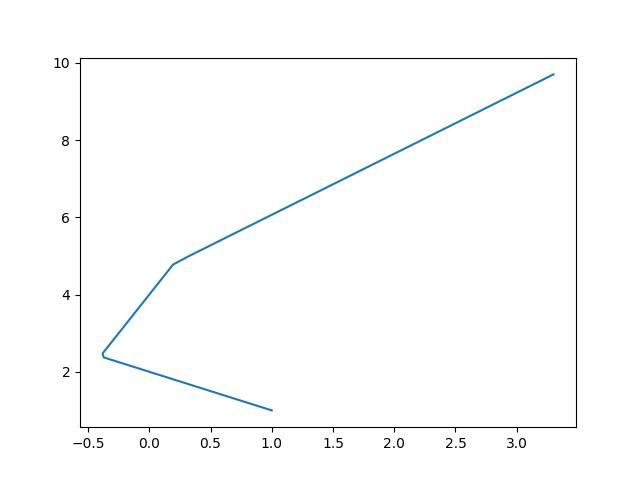
\includegraphics[width=25em]{calc_multi_75_app_09.jpg}

Başlangıcı $a_x,a_y$ olan kesik bir eğriyi görüyoruz. Bu tür eğrileri aynen
[6]'da olduğu gibi sigmoid bazlı yapabiliriz,

\begin{minted}[fontsize=\footnotesize]{python}
rho = 7.0
def sig(x,a):
   return (x-a)*1/(1+np.exp(-rho*(x-a)))

def maxk(x,a):
   return np.max([0,x-a])

ax,bx,cx,dx,ex = (1, 2.4, 1, -3.5, -2.1)
ay,by,cy,dy,ey = (1, 0.4, -0.1, 0.5, -3)
def f(t):
    x = ax + \
        bx*maxk(t,2) + \
        cx*maxk(t,3) + \
        dx*maxk(t,3.5) + \
        ex*maxk(t,4.0)
	   
    y = ay + \
        by*maxk(t,2) + \
        cy*maxk(t,3) + \
        dy*maxk(t,3.5) + \
        ey*maxk(t,4.0)
    return x,y	   
    
def g(t):
    x = ax + \
        bx*sig(t,2) + \
        cx*sig(t,3) + \
        dx*sig(t,3.5) + \
        ex*sig(t,4.0)
	   
    y = ay + \
        by*sig(t,2) + \
        cy*sig(t,3) + \
        dy*sig(t,3.5) + \
        ey*sig(t,4.0)
    return x,y	   
    
tmp = np.linspace(0,5,100)
\end{minted}

\begin{minted}[fontsize=\footnotesize]{python}
res = np.array([f(tt) for tt in tmp])
plt.plot(res[:,0],res[:,1])
plt.savefig('calc_multi_75_app_10.jpg')
\end{minted}

\begin{minted}[fontsize=\footnotesize]{python}
res = np.array([g(tt) for tt in tmp])
plt.plot(res[:,0],res[:,1])
plt.savefig('calc_multi_75_app_11.jpg')
\end{minted}

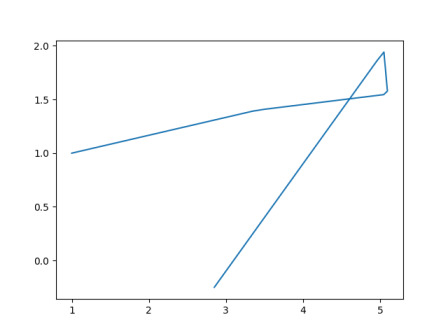
\includegraphics[width=20em]{calc_multi_75_app_10.jpg}
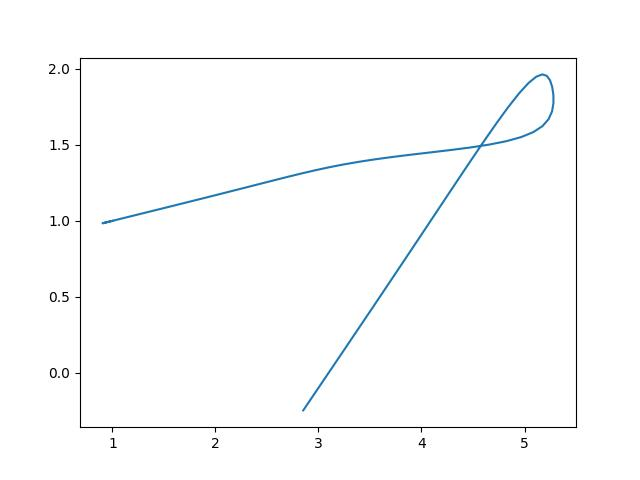
\includegraphics[width=20em]{calc_multi_75_app_11.jpg}

Herhangi bir şekli katsayılarla yaratmak mümkün. 

Bitiş noktalasını nasıl ayarlarız? Burada yine polinom örnekteki gibi
cebirsel bir yöntem seçebilirdik, fakat çoğunlukla başlangıç ve bitiş
arasındaki eğriler bir optimizasyon bağlamında kullanılır. Bu durumda
bitiş noktaları ile katsayılar arasında bir optimizasyon kısıtlaması
yaratmak ve bitiş noktalarını böyle ayarlamak daha iyidir. 

Çünkü biliyoruz parametrize ortamda mesela önceki örnekte $0 \ge t \ge
5$. O zaman egrinin bitisinde $t=5$ olacağını biliyoruz. Bu durumda mesela 

$$
    x = a_x + \
        b_x \sigma(t,2) + \
        c_x \sigma(t,3) + \
        d_x \sigma(t,3.5) +
        e_x \sigma(t,4.0)
$$

ifadesine $t$ tüm ilmik noktalarının ötesinde olduğu için artık tüm
$\sigma$ ifadeleri 1 veriyor. Eğer 1 veriyorsa, yani tüm sigmoid'ler aktif
ise, eğri bitişinde bilinen $t$ üzerinden elimizdeki $x$ 
$x = a_x + b_x(5-2) + c_x(5-3) + d_x(5-3.5) + e_x(5-4.0)$
olmalı. Optimizasyonda bu eşitliğin belli bir değer (istediğimiz bitiş
noktası kordinatı) olmasını şart tutarak amacımız erişebiliriz.

Kaynaklar

[1] Marsden, {\em Vector Calculus}

[2] Strang, {\em Calculus Volume 3, OpenStaxa}

[3] Sunday, {\em Intersection of Lines and Planes}, 
\url{http://geomalgorithms.com/a05-_intersect-1.html}

[4] Khaled, {\em Straight Line and Plane Intersection Matlab Code}, 
\url{https://uk.mathworks.com/matlabcentral/fileexchange/17751-straight-line-and-plane-intersection}

[5] {\em Distance between Point and Line}, 
\url{https://brilliant.org/wiki/distance-between-point-and-line/}

[6] Bayramlı, {\em Hesapsal Bilim, Spline Eğrileri ve Baz Fonksiyonlar}

[7] Rotenberg, {\em CSE169: Computer Animation},
    \url{https://cseweb.ucsd.edu/classes/wi19/cse169-a/slides/}

[8] Bayramlı, {\em Cok Degiskenli Calculus - Ders 4}
    
\end{document}

